\section{Targets}
 The areal density of scattering centers ( in $\mathrm{cm^{-2}}$) in Eq.~\eqref{eqxs_org} is calculated from the known target thickness:
\begin{equation}
  \eta_{tg} = \frac{\rho\cdot l \cdot N_{a}}{A},
  \label{eq_ntg}
\end{equation}
where $\rho$ is the density of the target material in $\mathrm{g/cm^{3}}$, $l$ is the effective target length in \emph{cm}, $N_{a}$ is the Avogadro's number and A is the nuclear number of the target.
behaviour
\subsection{Cryo-Target Boiling Effect}
\begin{figure}[!ht]
  \begin{center}
    \subfloat[$^{2}H$]{
      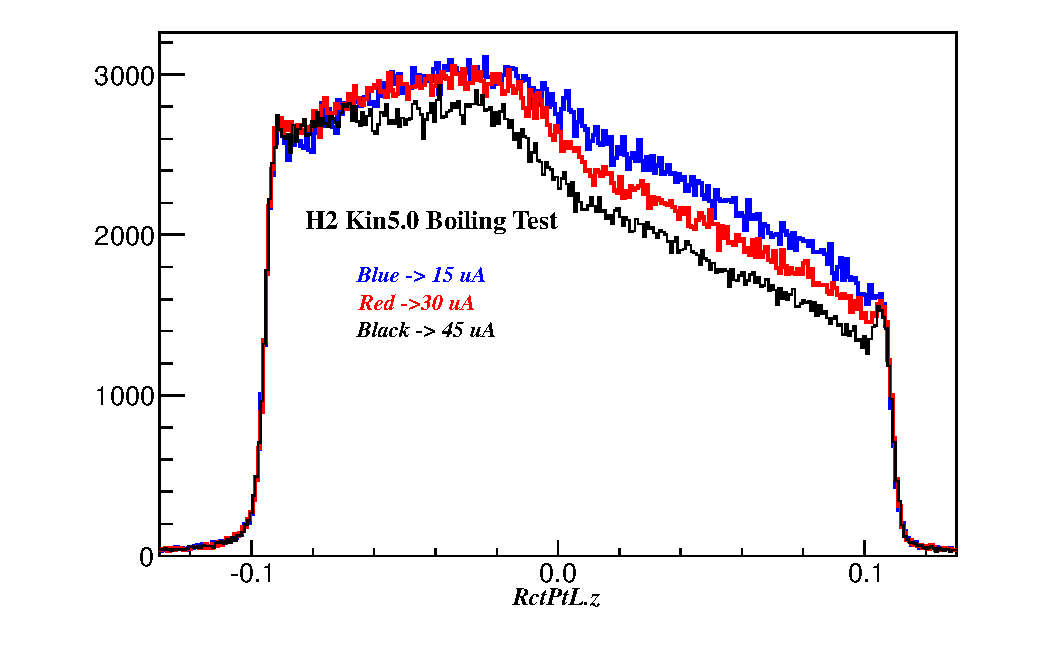
\includegraphics[type=pdf, ext=.pdf,read=.pdf,width=0.62\textwidth]{./figures/target/H2_Boiling_VZ}
    }
    \\
    \subfloat[$^{3}He$]{
      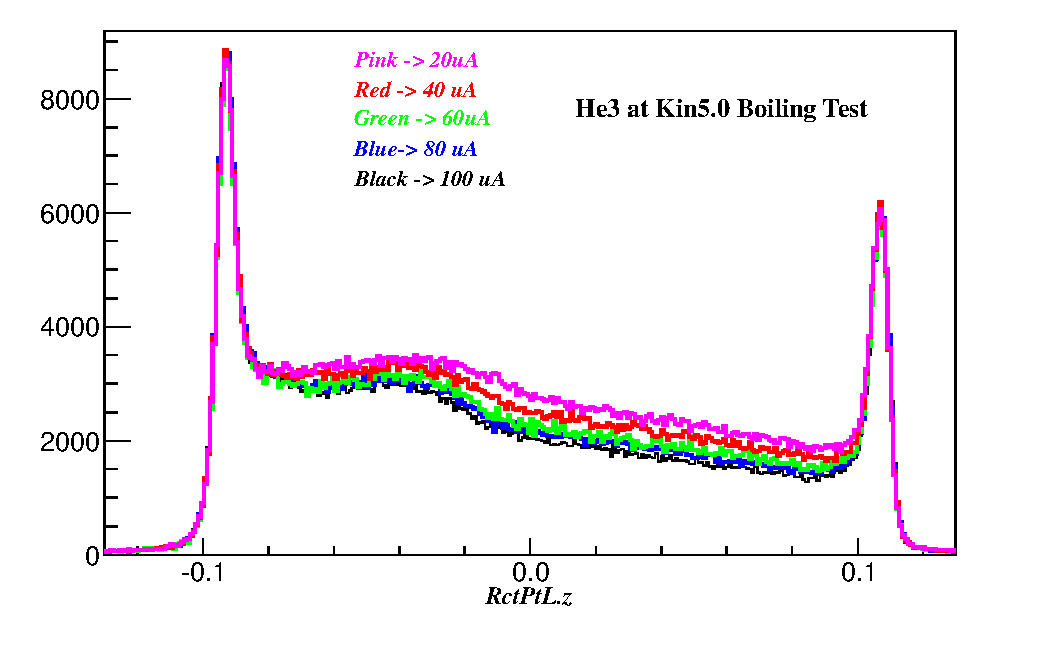
\includegraphics[type=pdf, ext=.pdf,read=.pdf,width=0.62\textwidth]{./figures/target/He3_Boiling_VZ}
    }
    \\
    \subfloat[$^{4}He$]{
      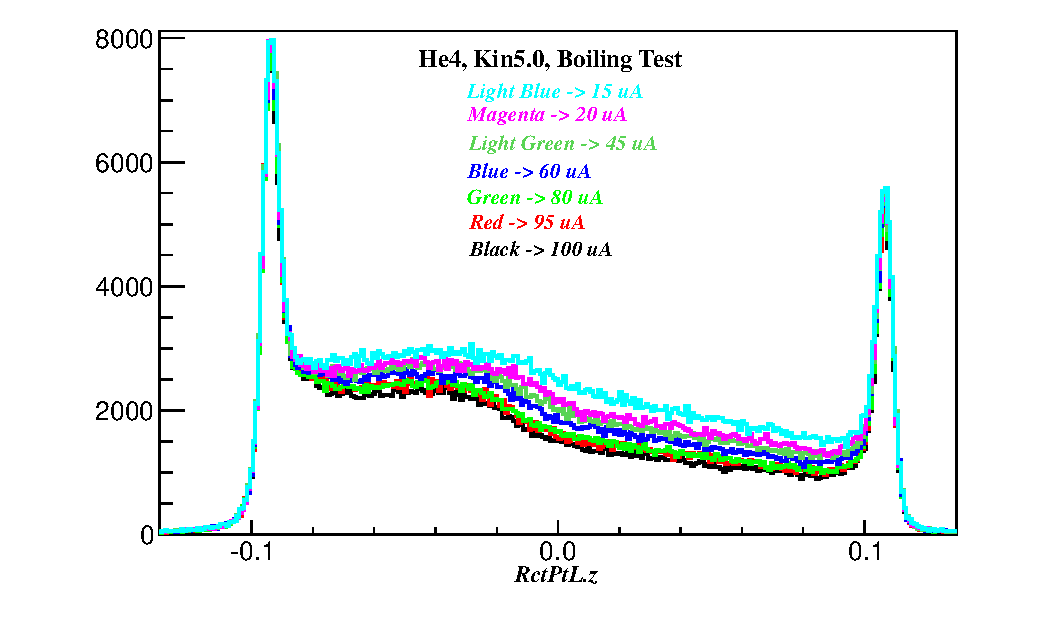
\includegraphics[type=pdf, ext=.pdf,read=.pdf,width=0.62\textwidth]{./figures/target/He4_Boiling_VZ}
    }
    \caption[Cryo-target bumps]{\footnotesize{Cryo-target bumps which appear on the $z_{react}$ distributions because of the non-uniform density of cryo-targets. Due to the boiling effect, the bumps become more significant when the beam current is larger.}}
    \label{bump_current}
  \end{center}
\end{figure}
 When the electron beam passes through the target, the local temperature fluctuates and causes the target density to vary with the beam current. This phenomenon is called the boiling effect. While the density variation of solid targets is usually negligible, liquid and gas targets have significant boiling effects and their densities correlate to the beam current as follow:
\begin{equation}
  \rho = \rho_{0} \cdot (1.0 - B \cdot I /100),
  \label{eq_tgrho}
\end{equation}
where $I$ and $B$ are the values of the beam current and the boiling factor for the target, respectively. $\rho_{0}$ is the nominal target density at $I=0$ and $\rho$ is the actual density with the boiling effect.

 In the E08-014, three cryogenic targets (cryo-targets), $\mathrm{^{2}H}$, $\mathrm{^{3}He}$ and $\mathrm{^{4}He}$, were held in 20 cm long aluminium cells. The cryogenic coolant flowed from the upstream to the downstream of a target cell, and the variation of temperature among different parts of the target leaded to a non-uniform density distribution. When the beam was on, the temperature fluctuation became more significant with higher current. The boiling effect was different along the cryo-target and further increased the non-uniformity of the target densities. Fig.~\ref{bump_current} shows the irregular density distribution and the strong correlation between the density and the beam current. The areal density, $\eta_{tg}$, for these cryo-targets could not be simply calculated from Eq.~\eqref{eq_ntg}.

  A boiling study was performed by dividing each target into several sections along the cell, where the boiling effect was individually evaluated. The relative density distributions were extrapolated from the boiling study results and the absolute target densities were calculated with the survey report of the target system~\cite{target_report}. A detailed discussion is given in Appendix D. 
 
% \subsection{Cryo-Target Cell Contamination}